%!TEX root = paper.tex

\begin{figure}[t]

\begin{subfigure}[t]{\columnwidth}
\begin{center}
\scalebox{1}{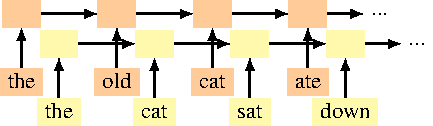
\includegraphics{CompiledTikzPictures/paper-figure0.pdf}}
\end{center}


\caption{\label{fig:batching:good}A conventional sequence-based RNN for two sentences.}
\end{subfigure}

\begin{subfigure}[t]{\columnwidth}
\begin{center}
\scalebox{1}{
 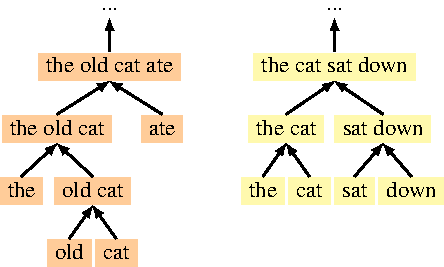
\includegraphics{CompiledTikzPictures/paper-figure1.pdf}}
\end{center}

\caption{\label{fig:batching:bad}A conventional TreeRNN for two sentences.}
\end{subfigure}

\caption{\label{fig:batching} An illustration of two standard designs for sentence encoders. The TreeRNN, unlike the sequence-based RNN, requires a substantially different connection structure for each sentence, making batched computation impractical.}
\end{figure}
